
The skew quadrupole geometry is presented in Fig. \ref{fig:Skew_quad_geometry}. Its two half-quadrants of two separate quadrants are positioned in one mechanical support. The entire magnet is then placed inside of the iron yoke. 
\begin{figure}[h!]
    \centering
    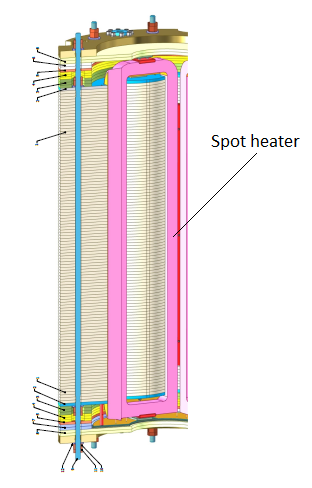
\includegraphics[width=0.25\linewidth]{figures/corrector_geometries/SpotHeaterPosition.png}
    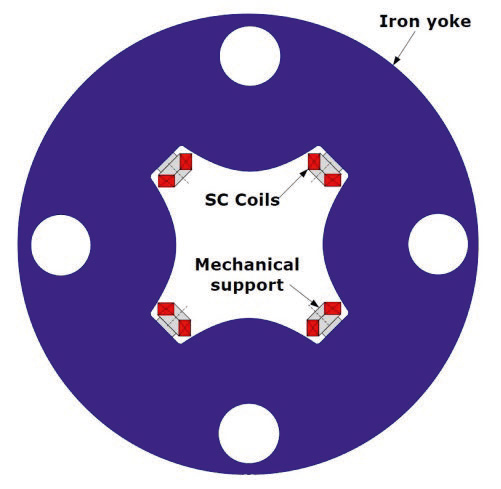
\includegraphics[width=0.30\linewidth]{figures/corrector_geometries/Quadrupole_Cross_Section.png}
    \caption{Left: quarter of skew quad 3D geometry; right: cross-section of skew quadrupole \cite{hl_lhc_tech_design_report_v01}}
    \label{fig:Skew_quad_geometry}
\end{figure}
Each quadrant of the magnet consists of 754 windings, as shown in Fig. \ref{fig:Skew_quad_cross_section}. There are 29 of them in each of 26 layers. When 3D analysis of a magnet is considered, it is important to specify the reeling scheme which allows for defining turn-to-turn quench propagation in a proper manner. In each quadrant, reeling starts at the bottom left of the cross-section and then continues as described in Fig. \ref{fig:Skew_quad_cross_section}. The \nth{2} half of each quadrant is a mirror reflection of the presented reeling scheme.

\begin{figure}[h!]
    \centering
    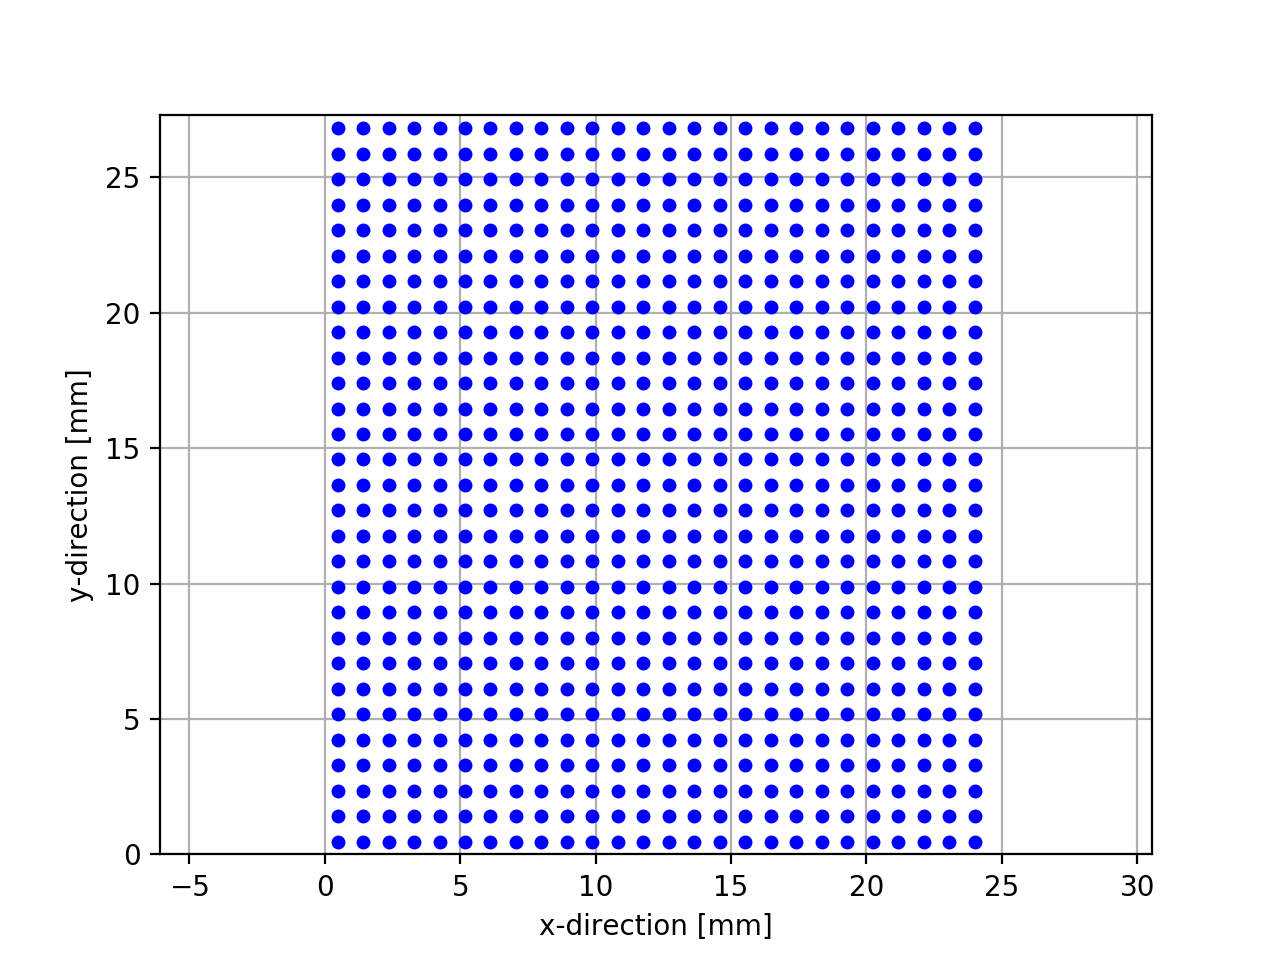
\includegraphics[width=0.49\linewidth]{figures/skew_quad_bcs/magnetic_field_mapping/Quadrupole_Winding_Map_plot.png}
    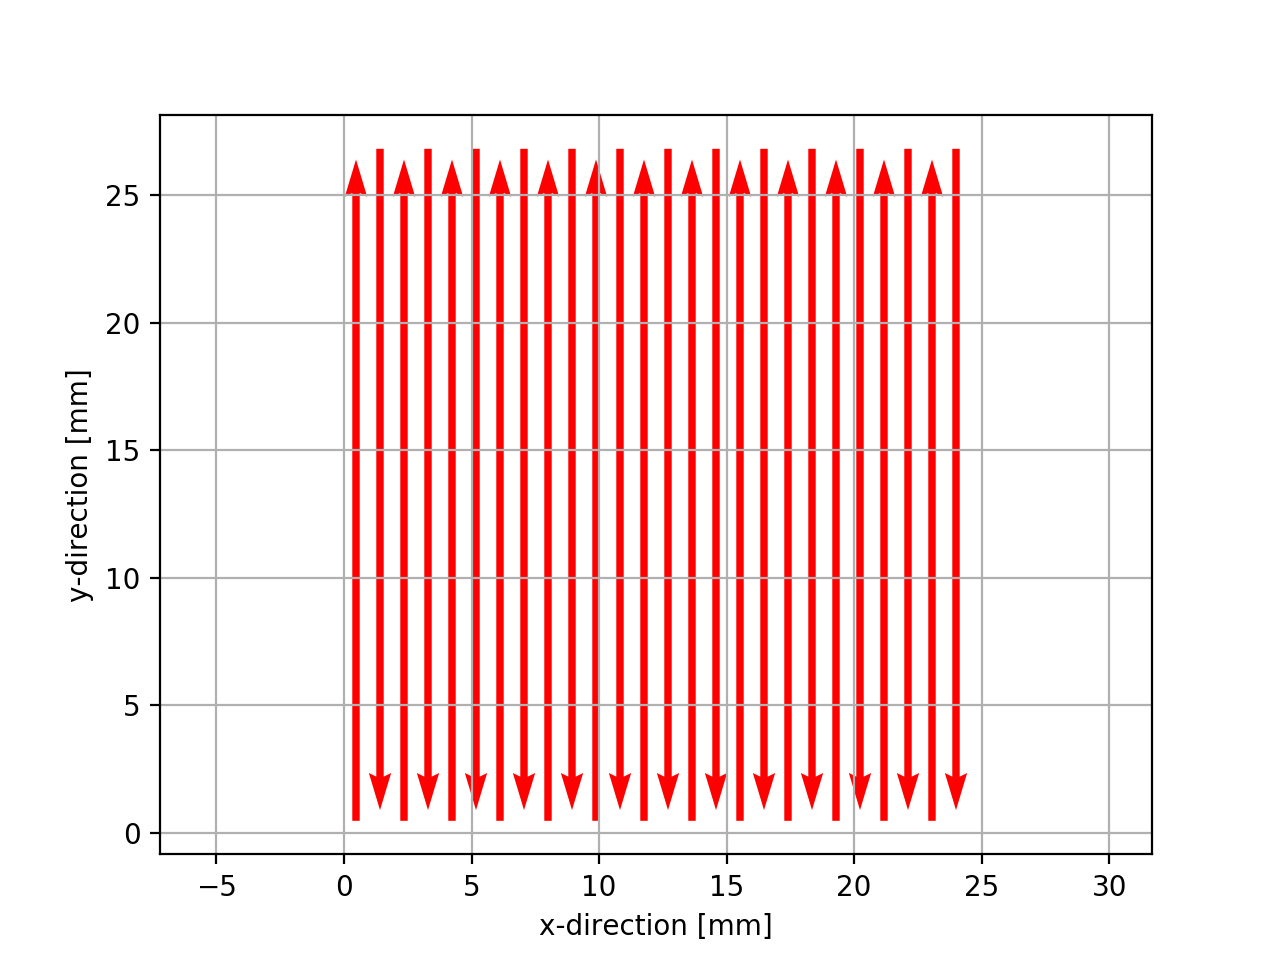
\includegraphics[width=0.49\linewidth]{figures/skew_quad_bcs/magnetic_field_mapping/Winding_Scheme.png}
    
    \caption{Left: location of windings in the same cross-section; right: reeling magnet scheme}
    \label{fig:Skew_quad_cross_section}
\end{figure}